\begin{figure}[H]
  \centering
  
  \begin{subfigure}[b]{0.3\textwidth}
    %% based on https://tex.stackexchange.com/questions/488865/3d-volume-in-tikz/488869#488869

\tdplotsetmaincoords{60}{110}
\begin{tikzpicture}[
  tdplot_main_coords,
  >= stealth,
  declare function = {
    pfft(\x) = pi + 0.3 * sin(deg(\x));
  }
]
  \draw[->] (0, 0, 0) coordinate (O) -- (4, 0, 0) coordinate(X)
    node[pos = 1.1] {\(x\)};
  \draw[->] (O) -- (0, 3, 0)
    node[pos = 1.1] {\(y\)};
  % \draw[->] (O) -- (0, 0, 4)
  %   node[pos = 1.1] {\(z\)};

  \draw plot[
    variable = \x,
    domain = 0.3 * pi : 0.9 * pi
  ] (3.0, \x, { pfft(2 * \x) }) coordinate (T1)
  -- plot[
    variable = \x,
    domain = 0.9 * pi : 0.3 * pi
  ] (0.8, \x, { pfft(2 * \x) }) coordinate (T3)
  -- cycle;

  \draw[dashed]
    (3, 0.3 * pi, 0) coordinate (B4)
    -- (3, 0.9 * pi, 0) coordinate (B1);
  \draw[dashed]
    (0.8, 0.9 * pi, 0) coordinate (B2)
    -- (0.8, 0.3 * pi, 0) coordinate (B3);
  \draw[dashed] (B1) -- (B2)
    node[midway, below, sloped] {\(\dd x\)};
  \draw[dashed] (B4) -- (B3);
  \path (B1) -- (B4)
    node[midway, below, sloped] {\(\dd y\)};

  \path (3, 0.3 * pi, { pfft(2 * 0.3 * pi) }) coordinate (T4)
    (0.8, 0.9 * pi,{ pfft(2 * 0.9 * pi) }) coordinate (T2);

  % \foreach \X in {1, ..., 4} {
  %   \draw[dashed] (B\X) -- (T\X);
  % }

  \path[
    opacity = 0.3,
    left color = blue,
    right color = blue,
    middle color = blue!20,
    shading angle = 72
  ] plot[
    variable = \x,
    domain = 0 : 1.1 * pi,
    smooth
  ] (3.5, \x, { pfft(2 * \x) })
  -- plot[
    variable = \x,
    domain = 1.1 * pi : 0,
    smooth
  ] (0, \x, { pfft(2 * \x) })
  -- cycle;

  \draw plot[
    variable = \x,
    domain = 0 : 1.1 * pi,
    smooth
  ] (3.5, \x, { pfft(2 * \x) })
  -- plot[
    variable = \x,
    domain = 1.1 * pi : 0,
    smooth
  ] (0, \x, { pfft(2 * \x) })
  -- cycle;

  \draw node at (1.9, 1.9, 0) {\(D_{xy}\)};
  \draw node at (1.3, 2.4, 2.9) {\(\dd \sigma\)};

  \draw[fill = black] (T4) circle (1pt);
  \draw[dashed, ->] (2, 0.4, 3) -- (4.3, 3.5, 2.8)
    node[pos = 0.7, below, sloped] {\(\vec{m_{1}}\)};
  \draw[dashed, ->] (3, 0.7, 3) -- (0.8, 0.7, 3.6)
    node[pos = 0.6, above, sloped] {\(\vec{m_{2}}\)};
\end{tikzpicture}

    \caption{В пространстве}\label{fig:proj_3}

  \end{subfigure}
  \qquad
  \begin{subfigure}[b]{0.3\textwidth}

    \input{figures/MI/14/proj_x.tex}
    \caption{\(x = const\)}\label{fig:proj_x}

  \end{subfigure}
  \qquad
  \begin{subfigure}[b]{0.3\textwidth}

    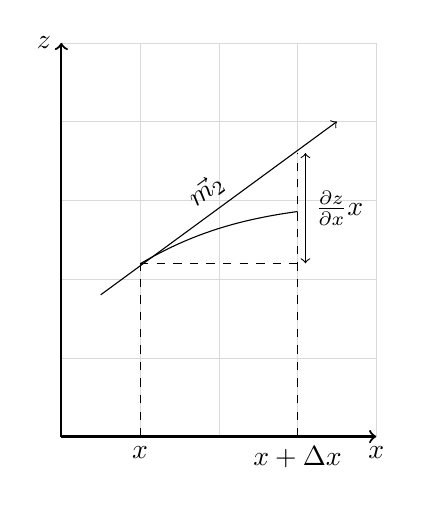
\begin{tikzpicture}
  \draw[very thin, gray!30, step = 1cm] (0, 0) grid (4, 5);
  \draw[domain = 1 : 3, variable = \x]
    plot ({\x}, {3 / (1 + e^(-\x))});

  \draw[thick] [->] (0, 0) -- (4, 0) node[right, below] {\(x\)};
  \draw[thick] [->] (0, 0) -- (0, 5) node[above, left] {\(z\)};

  \draw node[below] at (1, 0) {\(x\)};
  \draw node[below] at (3, 0) {\(x + \Delta x\)};

  \draw[dashed] (1, 0) -- (1, 2.2);
  \draw[dashed] (3, 0) -- (3, 3.6);

  \draw[dashed] (1, 2.2) -- (3, 2.2);
  \draw[<->] (3.1, 2.2) -- (3.1, 3.6)
    node[midway, right] {\(\frac{\partial z}{\partial x} \dd x\)};

  \draw[->] (0.5, 1.8) -- (3.5, 4)
    node[midway, above, sloped] {\(\vec{m_{2}}\)};
\end{tikzpicture}

    \caption{\(y = const\)}\label{fig:proj_y}

  \end{subfigure}
\end{figure}
